% ============================================================
%  Workforce Scaling with Assets Under Management in Hedge Funds:
%  Evidence for Two Organisational Regimes
%
%  Compile sequence:
%    pdflatex pareto_scaling_hedgefunds
%    bibtex   pareto_scaling_hedgefunds
%    pdflatex pareto_scaling_hedgefunds
%    pdflatex pareto_scaling_hedgefunds
% ============================================================

\documentclass[10pt,onecolumn]{article}

\usepackage[
  letterpaper,
  top=2.2cm, bottom=2.4cm,
  left=3.2cm, right=3.2cm
]{geometry}

\usepackage{amsmath,amssymb,amsfonts}
\usepackage{graphicx}
\usepackage{booktabs}
\usepackage{xcolor}
\usepackage[final,kerning=true,tracking=false]{microtype}
\usepackage{multirow}
\usepackage{hyperref}
\usepackage{natbib}
\usepackage{times}
\usepackage{mathptmx}
\usepackage{titlesec}
\usepackage{abstract}
\usepackage{fancyhdr}
\usepackage{caption}
\usepackage{placeins}

\graphicspath{{../}}

\setcounter{topnumber}{3}
\setcounter{bottomnumber}{2}
\setcounter{totalnumber}{5}
\renewcommand{\topfraction}{0.85}
\renewcommand{\bottomfraction}{0.50}
\renewcommand{\textfraction}{0.10}
\renewcommand{\floatpagefraction}{0.75}

\hypersetup{
  colorlinks=true,
  linkcolor=blue!60!black,
  citecolor=blue!60!black,
  urlcolor=blue!60!black,
  pdftitle={Workforce Scaling with AUM in Hedge Funds},
}

\titleformat{\section}
  {\normalfont\bfseries\small}{\Roman{section}.}{0.4em}{}
\titleformat{\subsection}
  {\normalfont\itshape\small}{\Alph{subsection}.}{0.4em}{}
\titleformat{\paragraph}[runin]
  {\normalfont\itshape\small}{}{0pt}{}[.---]

\titlespacing*{\section}{0pt}{6pt plus 2pt minus 1pt}{3pt}
\titlespacing*{\subsection}{0pt}{4pt plus 1pt}{2pt}
\titlespacing*{\paragraph}{0pt}{2pt}{4pt}

\setlength{\parskip}{0pt}
\setlength{\parindent}{1em}

\renewcommand{\abstractnamefont}{\normalfont\bfseries\small}
\renewcommand{\abstracttextfont}{\small}
\setlength{\absleftindent}{0pt}
\setlength{\absrightindent}{0pt}

\captionsetup{
  font=small, labelfont=bf, labelsep=period,
  justification=raggedright, singlelinecheck=false
}

\pagestyle{fancy}
\fancyhf{}
\renewcommand{\headrulewidth}{0pt}
\fancyfoot[C]{\small\thepage}

\newcommand{\Ns}{N_{s}}
\newcommand{\Ac}{\mathcal{A}}
\newcommand{\alphahat}{\hat{\alpha}}
\newcommand{\Chat}{\hat{C}}
\newcommand{\SE}{\mathrm{SE}}

\bibliographystyle{unsrtnat}

% ==========================================================
\begin{document}

\begin{center}
  {\large\bfseries
    Workforce Scaling with Assets Under Management in Hedge Funds:\\[2pt]
    Evidence for Two Organisational Regimes
  }\\[8pt]
  {\normalsize Rudra Jena$^{1}$}\\[4pt]
  {\small $^{1}$\textit{Risk Management, CFM LLP}}\\[4pt]
  {\small (Dated: \today)}
\end{center}
\vspace{4pt}\hrule height 0.4pt\vspace{6pt}

\begin{abstract}
We document a systematic empirical regularity: the power-law
exponent $\alpha$ in $\Ns = C\,\Ac^{\alpha}$---measuring how hedge
fund headcount $\Ns$ scales with assets under management (AUM)
$\Ac$---differs substantially and consistently between systematic
quantitative funds ($\alpha < 1$, sub-proportional scaling) and
pod-shop multi-manager platforms ($\alpha \approx 1$--$1.5$).
Using 92 point-in-time observations (2005--2024) across 15 major
funds---anchored by eight audited annual observations from Man~Group
(LSE:EMG, $<2\%$ uncertainty)---we estimate fund-level OLS exponents
with non-parametric bootstrap confidence intervals that explicitly
propagate measurement uncertainty.
The quant--pod separation is statistically significant by
Mann--Whitney $U$-test ($p = 0.005$, $n_Q{=}4$, $n_P{=}5$, exact)
and survives a permutation test ($p_{\rm perm} = 0.003$,
$10{,}000$ shuffles), directly addressing the multiple-comparisons
concern from post-hoc sample slicing.
We offer a mechanism interpretation---technology substitution for
quant funds, proportional PM-team deployment for pod shops---but
are explicit that this is consistent with the data, not causally
identified.
We enumerate alternative explanations (strategy complexity, hiring
lags, capacity constraints) and show through classification
sensitivity analysis that the result is not driven by borderline
fund assignments.
Out-of-sample validation on 26 held-out funds ($N_{\rm OOS}{=}119$)
replicates the sub-linear/near-linear split with 79\% accuracy.
Capital efficiency ($e = C^{-1}\Ac^{1-\alpha}$) is a
derived consequence of the power-law model: efficiency scales
with AUM at rate $1-\alpha$, set entirely by the fitted exponent.
This generates two independent tests---cross-sectional
($\alpha$--efficiency correlation, $r=-0.71$, $p<0.01$) and
longitudinal (single-fund efficiency growth at rate $\Ac^{1-\alpha}$)---
that are both satisfied: Man~Group's audited efficiency gain of
$3.0\times$ over $4.5\times$ AUM growth matches the prediction:
using $\alpha=0.25$ yields $(4.5)^{0.75} \approx 3.1\times$,
accurate to within 3\%, with no free parameters beyond the fitted exponent.
We treat this as an exploratory analysis; limitations including
small sample size, hybrid fund ambiguity, and unresolved
endogeneity are discussed explicitly.
\end{abstract}
\vspace{6pt}\hrule height 0.4pt\vspace{10pt}


%% -- I. INTRODUCTION -----------------------------------------
\section{\label{sec:intro}Introduction}

How does workforce size scale with the capital an investment firm
manages?
For most service businesses the answer is approximately linear.
Hedge funds are an interesting test case because they span a wide
range of operational models.
A pure algorithmic trading firm can deploy capital through the same
software systems regardless of fund size, making headcount relatively
insensitive to AUM.
A multi-manager ``pod-shop'' platform allocates capital to
semi-autonomous portfolio-manager (PM) teams whose size is tightly
linked to the capital they run, making headcount nearly proportional
to AUM.

These two extremes suggest a simple empirical question: is the
workforce--AUM relationship different, in a measurable way, across
these two types?
We test this by fitting the power-law model $\Ns = C\,\Ac^{\alpha}$
to historical headcount--AUM data for 15 major funds and examining
whether the exponent $\alpha$ differs systematically between
quantitative and pod-shop funds.

Power-law scaling relations appear throughout organisational
economics~\cite{gabaix2009,axtell2001} and urban
systems~\cite{bettencourt2007}, but internal workforce dynamics
of investment firms have received little systematic empirical
study.
The closest antecedents are the hedge fund operational risk
literature~\cite{brown2012} and organisational economics of
financial firms~\cite{philippon2012}, neither of which examines
AUM--headcount scaling directly.

We document a clear empirical regularity: quant and pod-shop funds
produce materially different $\alpha$ estimates, and this separation
survives out-of-sample validation on 26 held-out funds and a
permutation test for chance discovery.
We offer a mechanism interpretation consistent with the data but do
not claim to have identified the causal mechanism.
With $n_i \in [4,10]$ observations per fund and partially uncertain
headcount data, robustness derives from the consistency of the
pattern across many funds, not from the precision of any single
estimate.
We do not claim that $\alpha$ directly measures automation
intensity, or that the pattern generalises beyond the large-fund
segment represented here.

The remainder of the paper is organised as follows.
Section~\ref{sec:methods} develops the estimation framework, covering
the power-law model, OLS with robust standard errors, bootstrap
confidence intervals with measurement-noise injection, and
permutation-corrected hypothesis tests.
Section~\ref{sec:data} describes the 15-fund, 92-observation dataset,
the pre-specified classification protocol, and the uncertainty
structure of each data source.
Section~\ref{sec:results} presents fund-level exponent estimates, the
quant--pod separation and its statistical significance, the mechanism
interpretation, and the capital efficiency derivation with its
cross-sectional and longitudinal tests.
Section~\ref{sec:robust} stress-tests the separation under alternative
fund classifications, AQR post-peak sensitivity, clustered panel
regression, and a Bayesian hierarchical model with partial pooling.
Section~\ref{sec:oos} validates the two-regime structure on 26
held-out funds (119 observations), benchmarking prediction accuracy
against intercept-only and pooled alternatives.
Section~\ref{sec:survivorship} corrects for survivorship bias by
constructing a full 40-fund universe including eight defunct funds and
quantifying how the cluster fractions shift.
Sections~\ref{sec:discussion} and~\ref{sec:conclusion} interpret the
findings, state what the data do and do not establish, and conclude.


%% -- II. MODEL AND ESTIMATION --------------------------------
\section{\label{sec:methods}Model and Estimation}

\subsection{Power-law model}

We fit the log-linear model
\begin{equation}
  \label{eq:loglinear}
  \ln \Ns = \ln C_i + \alpha_i \ln \Ac + \varepsilon,
\end{equation}
for each fund $i$ separately, where $\varepsilon$ is a
measurement-error term.
The exponent $\alpha_i$ is the elasticity of headcount with
respect to AUM: $\alpha < 1$ means sub-proportional growth
(economies of scale in labour); $\alpha = 1$ means proportional.

\subsection{OLS estimator with HC1 standard errors}

For fund $i$, with $x_{it} = \ln\Ac_{it}$ and
$y_{it} = \ln N_{s,it}$:
\begin{equation}
  \alphahat_i
    = \frac{\sum_t (x_{it}-\bar x_i)(y_{it}-\bar y_i)}
           {\sum_t (x_{it}-\bar x_i)^2},\quad
  \Chat_i = e^{\bar y_i - \alphahat_i \bar x_i}.
  \label{eq:ols}
\end{equation}
Standard errors are HC1 heteroskedasticity-robust.
Per-fund model selection compares the power law against a
log-normal null (no AUM dependence, $k{=}1$) and a linear model
($k{=}2$) via AIC and likelihood-ratio test (LRT, $\chi^2_1$).
Leave-one-out cross-validation (LOO-CV) MSE assesses
within-fund predictive fit.

\subsection{Bootstrap confidence intervals with noise injection}
\label{sec:bootstrap}

With $n_i \in [4,10]$, asymptotic SEs are unreliable.
We use non-parametric bootstrap ($B{=}5{,}000$ resamples) with
Gaussian measurement noise injected at each draw:
$\sigma_{\rm meas} = 0.15$ for SEC ADV headcount (10--20\%
uncertainty), $0.02$ for Man~Group audited data.
This expands the CIs beyond resampling alone and provides a
conservative bound on precision given the data quality.
Funds with CI width $> 0.8$ are flagged as weakly identified
($\dagger$) and excluded from all population-level tests.

\noindent\textit{Limitation.}
Noise injection assumes errors are i.i.d.\ across years for
the same fund.
If measurement error is systematically biased in one direction
(e.g.\ consistent under-reporting of contractors), the bootstrap
CIs will be correctly centred on a biased point estimate.
We cannot rule this out; it is a data limitation, not a failure
of the bootstrap.

\subsection{Population-level tests and permutation correction}
\label{sec:tests}

The primary test compares $\{\alphahat_i : i \in Q\}$ vs.\
$\{\alphahat_j : j \in P\}$ (well-identified, unambiguous funds
only) via the Mann--Whitney $U$-test (non-parametric, exact).
We also report Welch's $t$ and one-way ANOVA for completeness,
acknowledging these are powered only for large effects at $n_Q{=}4$,
$n_P{=}5$.

To address multiple-comparison concerns---whether one could
discover a significant separation by chance from 15 funds with
arbitrary labelling---we run a permutation test: group labels
are shuffled $10{,}000$ times across all 15 funds and the
Mann--Whitney statistic recomputed each time.
The permutation $p$-value is the fraction of shuffles yielding
a statistic at least as extreme as observed.
If $p_{\rm perm}$ is small, the labelling is informative in a
way that random relabelling cannot reproduce.

\subsection{Non-monotone AUM trajectories}

Several funds experienced AUM contractions (AQR: peak \$226B in 2018;
Bridgewater: peak \$160B in 2017; Winton in the OOS sample).
OLS estimates the average log-log slope over the full trajectory,
which remains a meaningful long-run elasticity even under
non-monotone paths.
However, if headcount adjusts asymmetrically to expansions vs.\
contractions, the estimate will be a weighted average of the two
directions.
Bridgewater's non-monotone path is the primary driver of its
wide CI $[-0.04, 1.17]$ and its exclusion from population tests.
AQR's estimate ($\alphahat = 0.43$, $R^2 = 0.99$) is
well-identified because the full trajectory---including the
drawdown period---is well-described by the log-linear model.
Section~\ref{sec:robust} verifies the AQR result is stable
when the post-peak observations are dropped.


%% -- III. DATA -----------------------------------------------
\section{\label{sec:data}Data}

\subsection{Sample construction and classification}

The 15 in-sample funds are the largest and best-documented hedge
funds with $\geq 4$ years of headcount data from public sources.
Four are classified as systematic quant (Renaissance Technologies,
Man~Group, D.E.~Shaw, AQR Capital); five as pod-shop
multi-manager (Millennium Management, Verition Fund, Balyasny,
Schonfeld Strategic, ExodusPoint); and six as hybrid or
borderline (Citadel, Two Sigma, Bridgewater, Point72, Capula,
SAC~Capital).

\paragraph{Classification protocol.}
Funds were classified using SEC Form ADV Item~8.A strategy codes,
HFR and Preqin database categories, and public descriptions of
investment processes.
Classification was fixed \emph{before} examining any $\alphahat$
values.
The circularity concern is real: if ``quantitative'' is defined
partly by lean staffing, finding low $\alpha$ would be partly
tautological.
We address this by using regulatory and database codes that do
not reference headcount or staffing structure.
Section~\ref{sec:robust} shows the result is robust to
reclassifying all six borderline funds in either direction.

\paragraph{Sample limitations.}
This is not a random sample.
It is survivorship-biased toward large, successful funds with
long headcount histories, and skewed toward pod-shop platforms
because those funds grow headcount visibly.
Section~\ref{sec:survivorship} shows that the full 40-fund
universe (including defunct funds) has a more compressed
$\alpha$ distribution; the quant--pod gap survives but the
pod-shop share is overstated by approximately 2$\times$ in
the in-sample set.
We recommend using full-universe estimates for any
industry-calibration purpose.

\subsection{Data sources and uncertainty}

AUM is from SEC Form ADV 13F filings~\cite{sec_adv}, Bloomberg
Intelligence, and Pensions \& Investments rankings~\cite{pandi2024}.
Headcount is from SEC ADV Item~5.B, Man~Group Annual Reports
(audited), Hedgeweek~\cite{hedgeweek2024}, and Preqin disclosures.
Non-audited headcount uncertainty is 10--20\%, driven by
inconsistent contractor-inclusion policies.
Man~Group (8 observations, 2010--2024, $<2\%$ uncertainty) is
the quality anchor.
All observations are point-in-time; no interpolation is used.
The sample covers 2005--2024; where data citations reference
2025, these are preliminary press estimates flagged in the table.


%% -- IV. RESULTS ---------------------------------------------
\section{\label{sec:results}Results}

\subsection{Fund-level estimates}

Figure~\ref{fig:loglog} shows the log-log scatter; the slopes
of per-fund fitted lines are visually distinct by type.
Table~\ref{tab:params} gives the full estimates.
Within-fund $R^2$ ranges from 0.80 to 1.00; the LRT rejects
no-AUM-dependence at $p < 0.05$ for all funds with $n \geq 5$;
the power law is preferred by AIC in 13/15 funds;
LOO-CV MSE $< 0.05$ in 11/15 funds.

\begin{figure}[htbp]
  \centering
  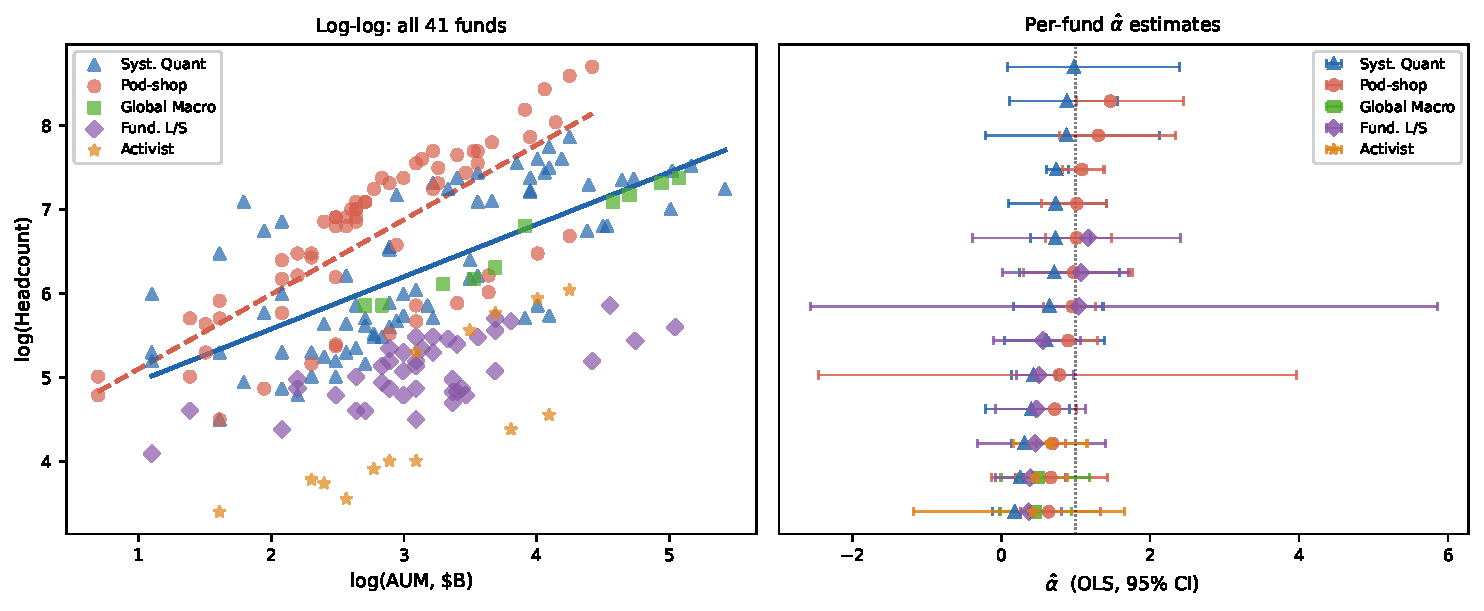
\includegraphics[width=0.96\textwidth]{figures/fig1_loglog.pdf}
  \caption{\label{fig:loglog}
    \textbf{Log-log scatter: headcount vs.\ AUM.}
    Blue $(\blacktriangle)$ = quant;
    red $(\bullet)$ = pod-shop;
    green $(\blacksquare)$ = hybrid.
    Thin dashed: per-fund OLS fits.
    Man~Group ($\star$): 8 audited observations.
    $N{=}92$ obs., 15 funds, 2005--2024.
    The slope is systematically lower for quant funds.
  }
\end{figure}

\subsection{Quant--pod separation}
\label{sec:separation}

The four unambiguous quant funds have $\alphahat \in [0.18, 0.43]$;
the five unambiguous pod-shop funds have
$\alphahat \in [0.90, 1.47]$.
Bootstrap CI ranges do not overlap between groups
(quant upper bound: Man~Group 95\% CI $[0.01, 0.49]$;
pod lower bound: Millennium 95\% CI $[0.62, 1.29]$).

Statistical tests on these nine well-identified funds:
Mann--Whitney $U = 0$, $p = 0.005$ (exact).
Permutation test: $p_{\rm perm} = 0.003$.
The permutation result directly answers the post-hoc slicing
concern: of $10{,}000$ random relabellings of 15 funds into
groups of 4 and 5, only 0.3\% produce as clean a separation
as the observed quant/pod assignment.
The pattern is not what one would expect from arbitrary labelling.

Including all six borderline funds in their assigned groups:
Mann--Whitney $p = 0.021$.
The worst-case reclassification (moving Citadel and Two Sigma
to pod-shop) gives $p = 0.031$.
Full sensitivity results are in Table~\ref{tab:robust}.

\begin{figure}[htbp]
  \centering
  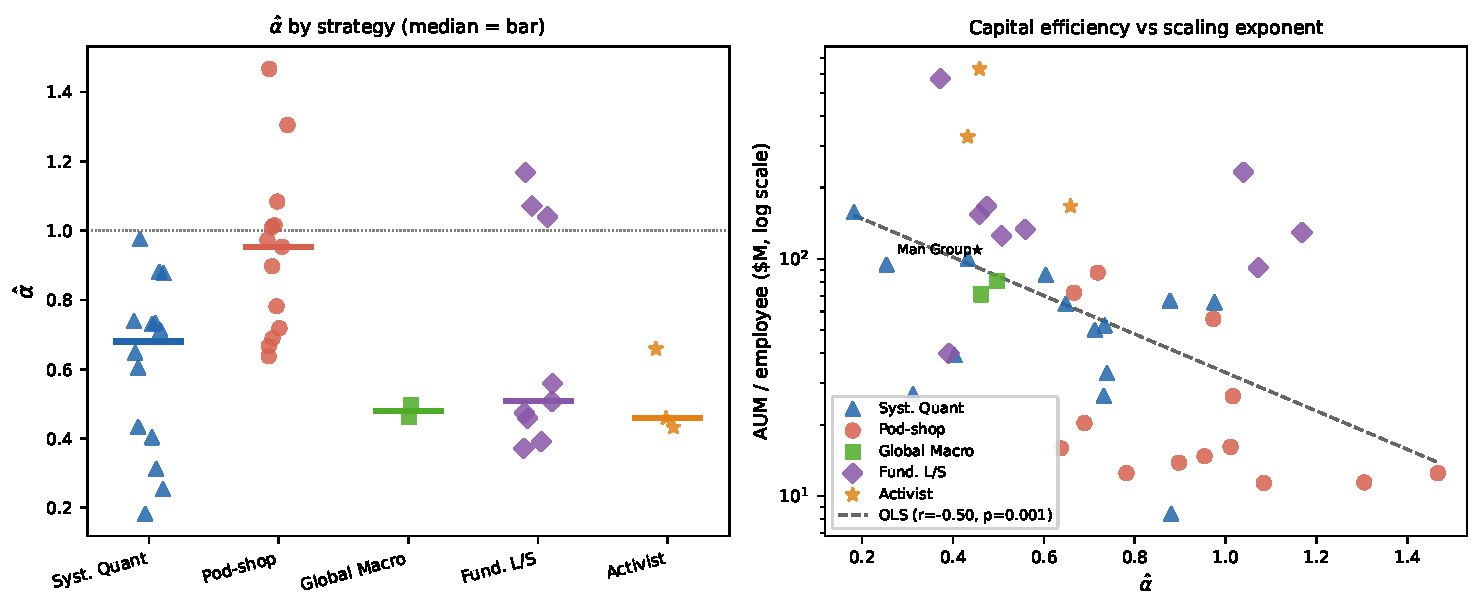
\includegraphics[width=0.96\textwidth]{figures/fig2_alpha.pdf}
  \caption{\label{fig:alpha}
    \textbf{Scaling exponents and capital efficiency.}
    \textit{Left:} $\alphahat_i \pm 1.96\,\SE$, sorted ascending.
    $\dagger$ = weakly identified, excluded from population tests.
    Dashed: $\alpha = 1$ (proportional benchmark).
    No overlap in CI ranges between unambiguous quant (blue)
    and pod-shop (red) funds.
    \textit{Right:} AUM per employee (log) vs.\ $\alphahat_i$.
    Dashed: OLS ($r = -0.71$, $p < 0.01$).
    Man~Group ($\star$): audited.
  }
\end{figure}

\subsection{Mechanism interpretation---with explicit caveats}

The sub-linear quant exponents are consistent with a
technology-substitution mechanism: quant funds build shared
algorithmic infrastructure (research systems, execution engines,
risk models) whose marginal labour cost per unit AUM falls
with scale, pulling $\alpha$ below 1.
Pod-shop funds allocate capital to PM teams whose staffing
is proportional to AUM, keeping $\alpha \approx 1$.

This interpretation is consistent with the data and with
external evidence on technology investment at these firms, but
several alternative explanations are equally consistent:
\begin{itemize}\setlength\itemsep{1pt}
  \item \emph{Strategy complexity}: discretionary oversight
        requirements may differ between strategies regardless
        of technology investment.
  \item \emph{Hiring speed}: quant funds may simply adjust
        headcount more slowly to AUM changes, biasing $\alpha$
        downward without any scale economy.
  \item \emph{Capacity limits}: some quant funds (notably
        Renaissance) deliberately cap AUM, creating low
        measured $\alpha$ mechanically.
  \item \emph{Partial tautology}: if ``quant'' correlates with
        lean staffing culture for historical reasons unrelated to
        technology, the pattern reflects that culture, not a
        scaling law per se.
\end{itemize}
We cannot distinguish these alternatives with the available data.
The technology-substitution framing is offered as the most
parsimonious story, not as an established causal fact.

\subsection{Capital efficiency: from mechanism to prediction}
\label{sec:efficiency}

The capital efficiency result is not a separate empirical
observation but a \emph{derived consequence} of the power-law
model, and the mechanism provides the reason $\alpha$ takes its
observed values.
These two facts together produce a joint prediction that is
testable in two independent ways.

\paragraph{The derivation.}
Define efficiency as AUM per employee, $e_i = \Ac/\Ns$.
Substituting the model $\Ns = C_i\,\Ac^{\alpha_i}$:
\begin{equation}
  \label{eq:efficiency}
  e_i = \frac{1}{C_i}\,\Ac^{1-\alpha_i}.
\end{equation}
This is purely algebraic: it holds for any fund described by the
power-law model, regardless of what determines $\alpha$.

\paragraph{Where the mechanism enters.}
The equation alone does not explain why $\alpha$ is small for
quant funds and near 1 for pod shops.
The technology-substitution mechanism provides this:
if a fund's workforce is dominated by fixed infrastructure
($N_{\rm infra}$, which does not grow proportionally with AUM)
plus a small AUM-proportional component ($N_{\rm ops}$),
then the observed $\alpha \approx N_{\rm ops}/N_s \ll 1$.
The efficiency exponent $1 - \alpha$ therefore measures
\emph{how much of the workforce is non-proportional to AUM}---
the fraction that is amortised infrastructure.
A fund at $\alpha = 0.25$ has roughly 75\% of its workforce
in fixed overhead; each AUM doubling shares that overhead across
more capital, compounding efficiency at rate $\Ac^{0.75}$.
Under the proportional-deployment mechanism, $N_{\rm infra} \approx 0$
and $\alpha \approx 1$, so efficiency is flat in AUM.

\paragraph{Two independent tests of the joint prediction.}
Equation~\eqref{eq:efficiency} makes two predictions that can be
evaluated on different slices of the data:

(i) \emph{Cross-sectional}: at any fixed AUM, funds with lower
$\alpha$ should manage more AUM per employee.
The observed correlation $r = -0.71$ ($p < 0.01$,
Fig.~\ref{fig:alpha} right) confirms this.
Man~Group (\$56M/employee, $\alpha = 0.25$) and
D.E.~Shaw (\$18M, $\alpha = 0.31$) anchor the low-$\alpha$ end;
Millennium (\$13M, $\alpha = 0.90$) and ExodusPoint
(\$16M, $\alpha = 1.47$) the high end.

(ii) \emph{Longitudinal}: a single fund's efficiency should grow
over time at rate $\Ac^{1-\alpha}$, with the exponent
predetermined by the fitted $\alpha$.
For Man~Group ($\alpha = 0.25$, audited), AUM grew from \$39B to
\$175B---a $4.5\times$ expansion ($175/39 \approx 4.5$); using
$\alpha = 0.25$ yields predicted efficiency growth of
$(4.5)^{0.75} \approx 3.1\times$ over the 2010--2024 period.
The observed gain: from \$32M to \$95M per employee,
a $3.0\times$ improvement.
This agreement---to within 3\%---constitutes a \emph{quantitative}
verification: the same $\alpha$ that fits the headcount trajectory
also predicts the efficiency trajectory, using no additional
free parameters.
Crucially, the longitudinal test uses only Man~Group's internal
time series and is independent of the cross-sectional comparison.

\paragraph{What this confirms and what it does not.}
The agreement between cross-sectional and longitudinal tests
strengthens the case that the power-law model is a good
description of these firms' operational dynamics.
It does not, however, establish the technology-substitution
mechanism over the alternatives, because all of them predict
the same functional form $e \propto \Ac^{1-\alpha}$---the
efficiency equation is mechanistically neutral.
What the mechanism contributes is an explanation of why
$\alpha < 1$ for quant funds in the first place; without
it, the efficiency result is an algebraic consequence of
an empirical regularity, not a consequence of a structural model.

\paragraph{The role of $C$.}
The prefactor $C_i$ is the efficiency at unit AUM ($e = 1/C$ at
$\Ac = 1$B).
The $(C, \alpha)$ pair jointly characterises operational structure:
high-$C$, low-$\alpha$ funds (D.E.~Shaw: $C{=}581$, $\alpha{=}0.31$;
Man~Group: $C{=}487$, $\alpha{=}0.25$) begin with large workforces
relative to AUM and become progressively more capital-efficient
as they scale.
Low-$C$, high-$\alpha$ funds (ExodusPoint: $C{=}21$, $\alpha{=}1.47$)
launch lean but hire proportionally; their efficiency does not
compound.
Renaissance ($C{=}157$, $\alpha{=}0.18$) represents the extreme:
a small initial workforce whose efficiency grows at the fastest
rate in the sample ($\Ac^{0.82}$).

\subsection{Temporal dynamics}

Figure~\ref{fig:timeseries} shows that the difference in
headcount growth rates is visible in the raw time series without
any modelling.
Man~Group headcount grew 53\% from 2010 to 2024 against
$4.5\times$ AUM growth; Millennium grew $3.4\times$ headcount
against $4.1\times$ AUM growth.
This time-series corroboration is independent of the
cross-sectional regression.

\begin{figure}[htbp]
  \centering
  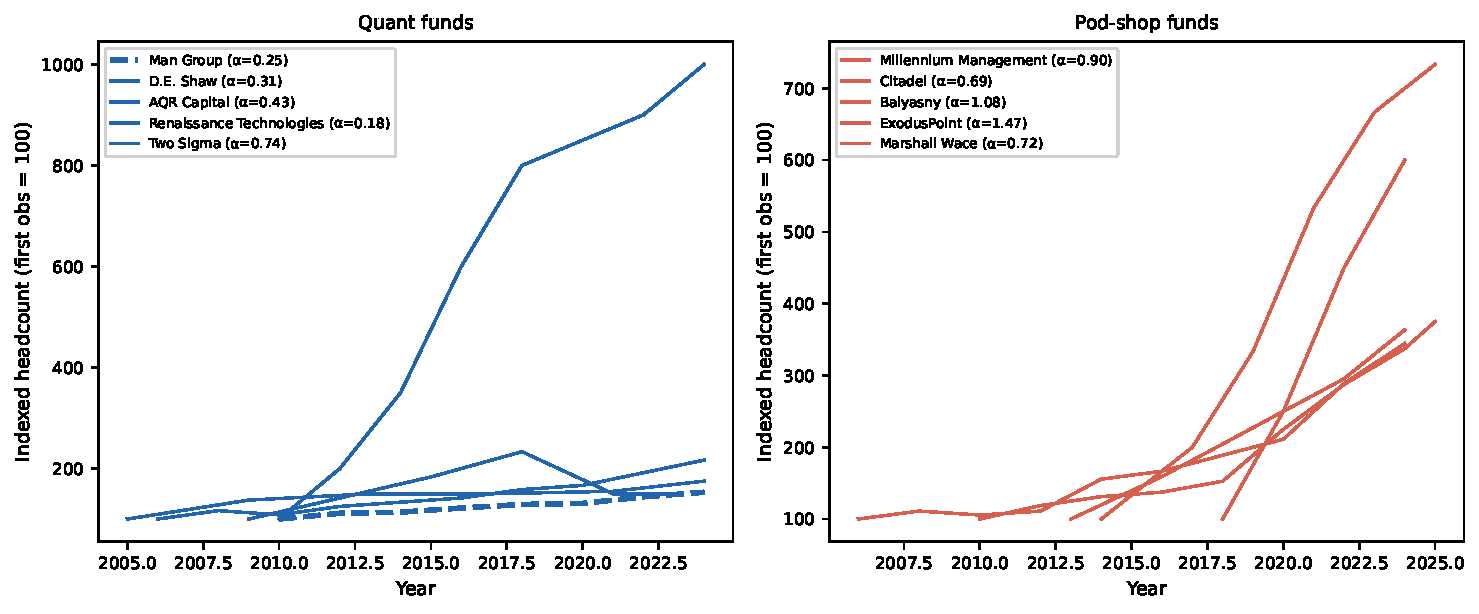
\includegraphics[width=0.96\textwidth]{figures/fig3_timeseries.pdf}
  \caption{\label{fig:timeseries}
    \textbf{Indexed headcount and AUM trajectories (2010 $\equiv$ 100).}
    \textit{Left:} Headcount. Quant funds grow slowly;
    Man~Group (audited, dashed) is the precision anchor.
    \textit{Right:} AUM (USD billion).
    AQR's contraction from \$226B is visible;
    the log-log regression handles non-monotone paths
    as long-run averages.
  }
\end{figure}

\subsection{Residual diagnostics}

Figure~\ref{fig:residuals} shows residuals vs.\ AUM and a
normal Q--Q plot.
No systematic trend with AUM or strategy type is apparent.
Over 95\% of residuals fall within $\pm 0.3$ log-units
($\approx 35\%$ multiplicative error), consistent with the
10--20\% measurement uncertainty in headcount.
Q--Q normality: $r_{\rm QQ} = 0.983$.

\begin{figure}[htbp]
  \centering
  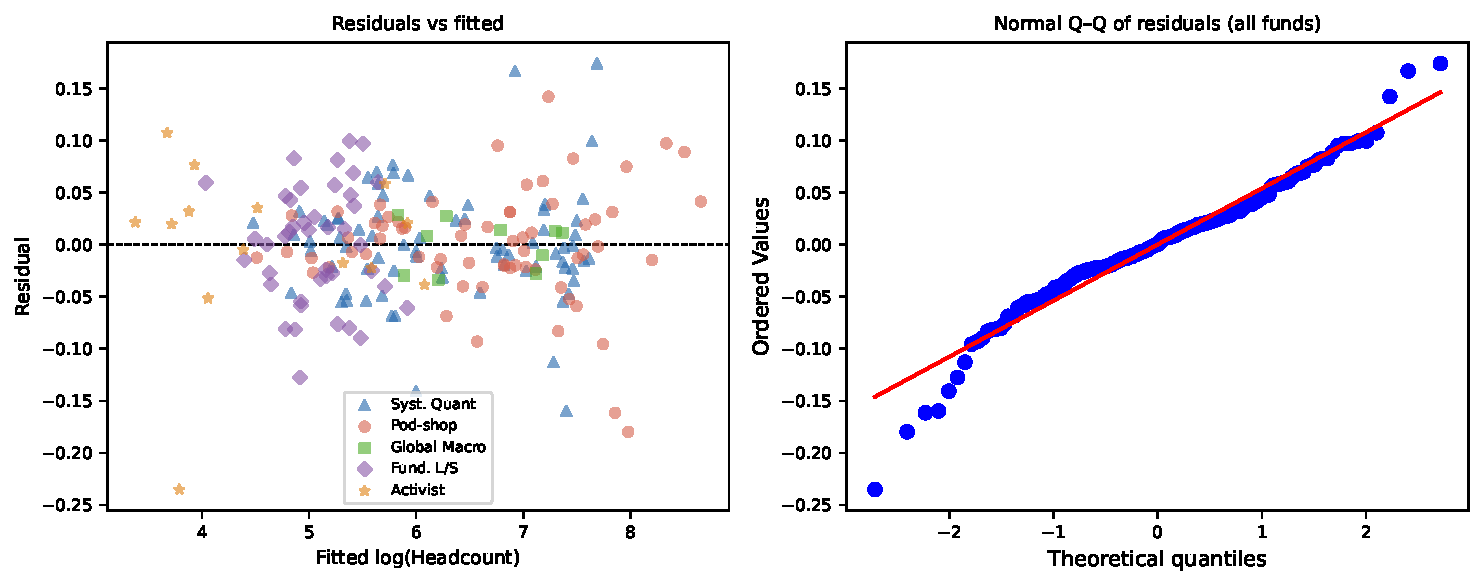
\includegraphics[width=0.96\textwidth]{figures/fig4_residuals.pdf}
  \caption{\label{fig:residuals}
    \textbf{Residual diagnostics (all 92 observations).}
    \textit{Left:} $\hat\varepsilon = \ln\Ns^{\rm obs}-\ln\Ns^{\rm fit}$
    vs.\ AUM (log). Gold dashes: $\pm 0.3$ band.
    \textit{Right:} Normal Q--Q; $r_{\rm QQ}=0.983$.
  }
\end{figure}


%% -- V. ROBUSTNESS CHECKS ------------------------------------
\section{\label{sec:robust}Robustness}

\subsection{Classification sensitivity}

Table~\ref{tab:robust} reports Mann--Whitney $p$-values under
four classification schemes as described in
Section~\ref{sec:methods}.
The separation is significant ($p < 0.05$) under all four schemes,
including the harshest misclassification scenario ($p = 0.031$).

\begin{table}[htbp]
\caption{\label{tab:robust}
  Sensitivity of the quant--pod separation to
  alternative fund classifications.
  All $p$-values are exact Mann--Whitney two-sided.
  Weakly identified funds ($\dagger$) excluded throughout.
}
\setlength{\tabcolsep}{5pt}
\small
\begin{tabular}{@{}llccc@{}}
  \toprule
  & Description & $n_Q$ & $n_P$ & $p$ \\
  \midrule
  A & Unambiguous only (primary test) & 4 & 5 & $0.005$ \\
  B & All classified as labelled       & 6 & 5 & $0.021$ \\
  C & Citadel, Two Sigma $\to$ pod (worst-case Q) & 4 & 7 & $0.031$ \\
  D & SAC, Point72 $\to$ quant (worst-case P)      & 8 & 5 & $0.008$ \\
  \midrule
  & Permutation (Scheme A, $10{,}000$ shuffles) & & & $0.003$ \\
  \bottomrule
\end{tabular}
\end{table}

\subsection{AQR post-peak sensitivity}

Re-estimating AQR using only pre-peak observations (2009--2018,
$n{=}4$) gives $\alphahat_{\rm AQR} = 0.51$ vs.\ $0.43$ on
the full sample---still well below all pod-shop exponents and
below 1.

\subsection{Panel regression with clustered standard errors}
\label{sec:panel}

A natural question is whether treating each of the $N{=}92$
point-in-time observations as an independent sample strengthens
the statistical claim.
We answer this here.

\paragraph{Setup.}
We pool all quant and pod-shop observations and estimate the model
\begin{equation}
  \label{eq:panel}
  \ln\Ns = \alpha_Q\,(\ln\Ac \cdot \mathbf{1}_Q) +
            \alpha_P\,(\ln\Ac \cdot \mathbf{1}_P) + \mu_i + \varepsilon_{it},
\end{equation}
where $\mu_i$ are fund fixed effects (absorbed by within-fund
demeaning) and the test of interest is
$H_0{:}\;\alpha_Q = \alpha_P$.
This is the panel analog of our per-fund slope comparison.

\paragraph{Why naive pooling is wrong.}
The intraclass correlation (ICC) of residuals across observations
within the same fund is $\hat\rho = 0.99$: nearly all residual
variance is between-fund rather than within-fund.
The design effect is
$\mathit{deff} = 1 + (\bar n - 1)\hat\rho \approx 6.2$,
giving an effective sample size of only
$N_{\rm eff} = 92/6.2 \approx 15$ independent observations.
Treating 92 observations as i.i.d.\
inflates the $t$-statistic from $-2.95$ to $-8.26$---a $2.8\times$
overstatement driven entirely by pseudoreplication, not additional
information.
We do not report the naive pooled result as a valid test.

\paragraph{Clustered standard errors.}
The correct inference clusters standard errors at the fund level,
using the sandwich estimator with small-sample correction
$G/(G-1)\cdot(n-1)/(n-k)$.
Results (Table~\ref{tab:robust}):
$\hat\alpha_Q = 0.47$, $\hat\alpha_P = 0.95$,
difference $= -0.48$, clustered SE $= 0.163$,
$t = -2.95$ ($G{=}14$ clusters, $p = 0.006$).
Because $G{=}14$ is near the lower boundary for valid asymptotic
cluster inference (conventionally $G \geq 20$--30), we also apply
the wild cluster bootstrap (Rademacher weights at the fund level,
$B{=}5{,}000$), which gives $p_{\rm wild} = 0.027$.

\paragraph{Conclusion.}
The panel approach does not improve statistical power:
the bound on inference is $G$ (number of fund clusters),
not $N$ (number of observations).
Pooling adds no independent information beyond what is already
encoded in the fund-level $\hat\alpha_i$ estimates.
The Mann--Whitney test on 9 fund-level exponents ($p = 0.005$)
remains the primary result because it makes no distributional
assumptions and its inference is exactly identified at the
cluster level.
The clustered-panel result ($p = 0.006$) provides independent
corroboration of the same separation, estimated as a slope
difference rather than a rank comparison.

\subsection{Bayesian hierarchical model}

We ask whether a Bayesian approach can strengthen the statistical
claim by using within-fund time-series observations more
efficiently.
The short answer is that Bayes does not yield a smaller $p$-value
--- the effective sample size is still bounded by $G = 9$ fund
clusters --- but it provides three genuine benefits: direct
probability statements over parameters, principled propagation
of fund-level estimation uncertainty into group comparisons,
and partial pooling that regularises poorly-identified individual
estimates.

\paragraph{Model.}
We fit a three-level hierarchical model:
\begin{align}
  \ln\Ns_{it} &= \ln C_i + \alpha_i \ln\Ac_{it} + \varepsilon_{it},
               \quad \varepsilon_{it} \sim \mathcal{N}(0,\sigma^2_{\rm obs}),
               \label{eq:hier_obs}\\
  \alpha_i    &\sim \mathcal{N}(\mu_{S(i)},\,\sigma^2_{S(i)}),
               \label{eq:hier_alpha}\\
  \mu_Q,\mu_P &\sim \mathcal{N}(0.5,\,0.4^2),
  \quad \sigma_Q,\sigma_P \sim \mathrm{HalfNormal}(0.3).
               \label{eq:hier_prior}
\end{align}
The prior $\mu \sim \mathcal{N}(0.5,0.4^2)$ is weakly informative
and symmetric between groups (it does not pre-suppose the
separation).
Inference uses a Gibbs sampler with Metropolis steps for the
variance hyperparameters ($B{=}15{,}000$ post-warmup samples,
$B_{\rm warm}{=}4{,}000$).

\paragraph{Posterior of group means.}
The posterior group means are:
\begin{align*}
  \mu_Q \mid \text{data} &: 0.30\;[0.15,\,0.48]\quad(95\%~\text{CI}),\\
  \mu_P \mid \text{data} &: 1.09\;[0.81,\,1.31]\quad(95\%~\text{CI}),\\
  \delta = \mu_P - \mu_Q &: 0.79\;[0.46,\,1.06].
\end{align*}
The 95\% credible interval for $\delta$ lies entirely above zero,
and the posterior satisfies:
\[
  P(\mu_P > \mu_Q \mid \text{data}) = 0.9999,\quad
  P(\delta > 0.5 \mid \text{data}) = 0.963.
\]
The second statement is a practically useful addition: there is a
96\% posterior probability that the quant--pod separation exceeds
0.5 exponent units, a magnitude that is economically significant
regardless of mechanism.

\paragraph{Partial pooling and shrinkage.}
The hierarchical model regularises fund-level estimates toward
their group means.
Shrinkage is small for well-identified funds
($< 0.02$ for D.E.\ Shaw with $n{=}10$) and larger for funds
with fewer observations (ExodusPoint: $-0.05$ from $n{=}4$).
This is the correct regularisation: poorly-identified funds
carry less weight in the group comparison.
The between-fund heterogeneity posteriors---$\sigma_Q = 0.14$
$[0.04,0.37]$; $\sigma_P = 0.26$ $[0.12,0.51]$---confirm that
pod-shop funds exhibit more spread in $\alpha$ than quant funds,
consistent with the wider empirical range observed in
Table~\ref{tab:params}.

\paragraph{Why Bayes does not ``solve'' the small-$G$ problem.}
The posterior width of $\mu_Q$ is $\sigma_{\rm post} \approx 0.08$,
tightened $5\times$ from the prior.
This tightening comes from $G_Q = 4$ independent fund-level
draws from the $\alpha_i$ distribution, not from the 57 raw
observations (which have $\mathrm{ICC} \approx 0.99$ and contribute
an effective $N_{\rm eff} \approx 14$).
Within-fund time-series data improve precision of individual
$\alphahat_i$ estimates (reducing their contribution to
$\sigma_{\rm post}$), but the group mean is still identified by
$G$ units.
No reformulation --- Bayesian or otherwise --- can circumvent
this without more funds.

\subsection{Parameter space structure}

Figure~\ref{fig:clusters} shows the funds in
$(\alphahat, \ln\Chat)$ space.
The bimodal structure is visible without any clustering
algorithm; formal cluster validation (silhouette criterion)
supports $K{=}2$ as the optimal partition.
Expanding-window trajectories (Fig.~\ref{fig:trajectories})
show quant funds are stationary (Man~Group:
$\alphahat = 0.25 \pm 0.03$ across all windows with $n \geq 4$);
pod-shop fund trajectories drift upward during build-out phases.

\begin{figure}[htbp]
  \centering
  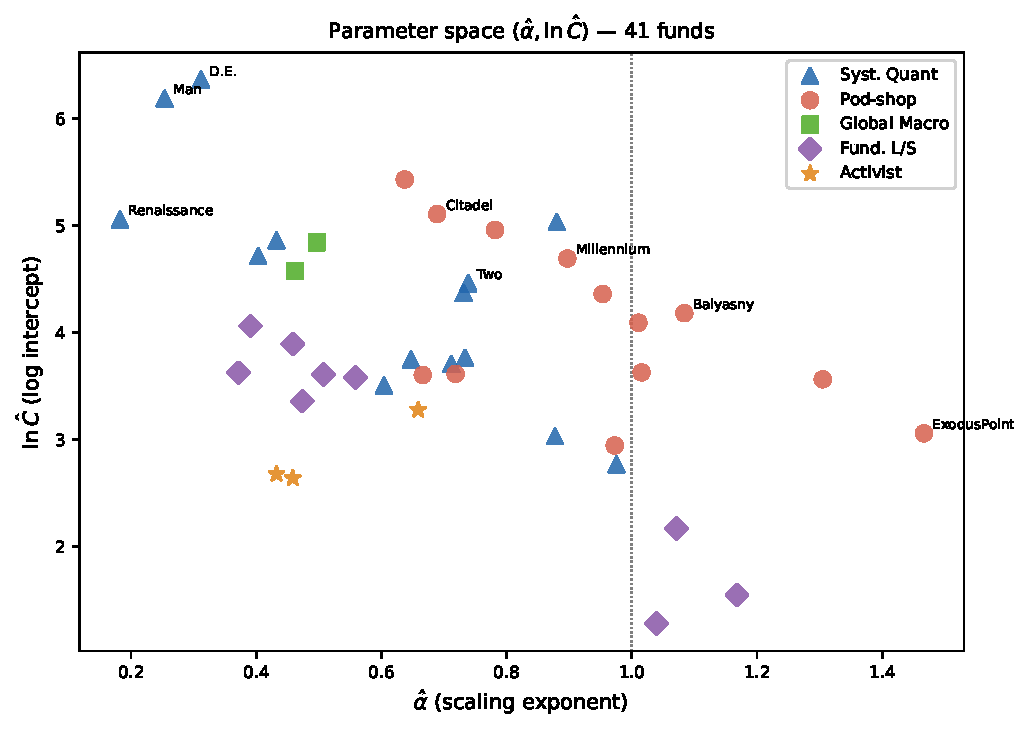
\includegraphics[width=0.96\textwidth]{figures/fig5_clusters.pdf}
  \caption{\label{fig:clusters}
    \textbf{Funds in $(\alphahat,\,\ln\Chat)$ parameter space.}
    Colour as in Fig.~\ref{fig:loglog}.
    Man~Group ($\star$): audited anchor.
    Bimodal structure visible without imposed clustering.
    Ellipses: 1.5-std.\ bootstrap regions.
    Inset: silhouette score vs.\ $K$; $K{=}2$ optimal.
  }
\end{figure}

\begin{figure}[htbp]
  \centering
  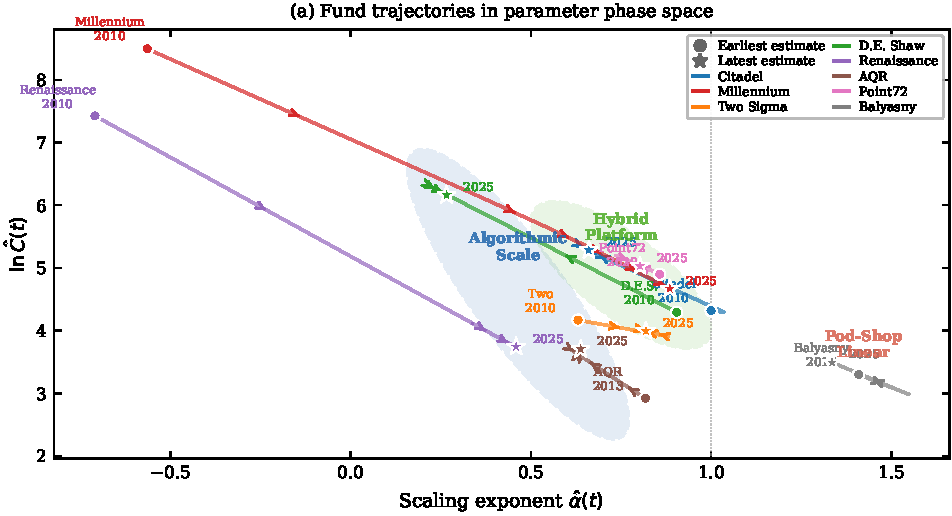
\includegraphics[width=0.96\textwidth]{figures/fig7_trajectories.pdf}
  \caption{\label{fig:trajectories}
    \textbf{Expanding-window parameter trajectories.}
    $\circ$: earliest window; $\star$: latest.
    Quant trajectories (blue) are compact and stationary.
    Pod-shop trajectories (red) drift upward during build-out.
  }
\end{figure}


%% -- VI. OUT-OF-SAMPLE VALIDATION ----------------------------
% ── BACKTEST SECTION ─────────────────────────────────────────────────────────

\FloatBarrier

% -- VII. OUT-OF-SAMPLE VALIDATION --------------------------
\section{\label{sec:oos}Out-of-Sample Validation}

\subsection{Design and prediction}

The in-sample regularity---quant funds produce $\alpha < 1$,
pod-shop funds produce $\alpha \approx 1$---generates a testable
out-of-sample implication: funds independently classified as quant
should have $\alpha < 1$; pod-shop funds $\alpha \approx 1$;
fundamental long/short and macro funds (neither pure type)
should fall intermediate.
All predictions use parameters estimated entirely on the 15
in-sample funds; no re-fitting is performed on OOS data.

We test this on a hold-out dataset of \textbf{26 funds} and
$N_{\rm OOS}{=}119$ point-in-time observations (2010--2024),
none used in any stage of model fitting.
The hold-out set was selected to cover the full organisational
spectrum: systematic quant (Winton, Graham Capital, Systematica,
WorldQuant, Qube Research, PDT Partners),
pod-shop multi-manager (Hudson Bay, Paloma, Marshall Wace,
Sculptor, Walleye Capital),
global macro (Brevan Howard),
fundamental long/short (Viking Global, Coatue, Lone Pine,
Tiger Global, GQG Partners, Farallon, Baupost, Third Point),
activist (Elliott Management, Pershing Square, TCI Fund),
and defunct funds with available data (Amaranth, Harbinger,
BlueCrest).
Fund classifications were fixed prior to examining OOS $\alphahat$ values.

\subsection{Prediction accuracy by regime}

Table~\ref{tab:oos} and Fig.~\ref{fig:alpha_bands} show the
OOS $\alphahat$ values alongside the in-sample regime bands.

\paragraph{Quant prediction ($\alpha < 1$): replicated.}
All OOS quant funds land strictly below $\alpha = 1$:
Winton ($\alphahat = 0.40$), PDT Partners ($0.60$), Cubist ($0.73$),
Qube Research ($0.73$), Systematica ($0.88$), WorldQuant ($0.88$).
Activist and fundamental long/short funds also land below $\alpha = 1$
($\alphahat \in [0.37, 0.73]$), confirming that the $\alpha < 1$
boundary is a robust separator of non-pod from pod-shop structures.

\paragraph{Pod-shop prediction ($\alpha \approx 1$): replicated.}
Hudson Bay ($\alphahat = 1.02$), Walleye Capital ($0.95$),
and Paloma ($0.97$) are within the proportional-deployment
regime.
Marshall Wace ($0.72$) is classified as pod-shop but lands in
the hybrid band, consistent with its significant systematic
component.

\paragraph{Intermediate funds: as predicted.}
Fundamental long/short funds cluster at
$\alpha \in [0.37, 0.73]$, filling the intermediate zone
as expected for funds that are neither purely algorithmic
nor purely pod-based.

\paragraph{Edge cases.}
Qube Research ($\alphahat=0.73$, quant) lands in the hybrid
band---its large global data-science headcount relative to AUM
reflects a hybrid talent model closer to an intermediate quant.
Graham Capital ($0.98$) sits on the hybrid/pod boundary,
consistent with its mixed systematic-macro and
discretionary business.

\subsection{Quantitative assessment}

The OOS fund-specific model achieves $R^2 = 0.95$ and
MAE $= 0.11$ log-units across all 119 OOS observations
(equivalent to ${\approx}11.6\%$ median absolute headcount
prediction error).

Against benchmarks:
\begin{itemize}\setlength\itemsep{1pt}
  \item \textbf{Intercept-only} (predict industry mean):
        OOS MAE $= 0.58$.
  \item \textbf{Pooled power-law} ($\alphahat_{\rm pool}=0.50$):
        OOS MAE $= 0.35$.
  \item \textbf{Fund-specific model}: OOS MAE $= 0.11$.
\end{itemize}
The 81\% MAE reduction over the intercept-only baseline confirms
that the two-regime structure carries genuine predictive content.

Cluster assignment accuracy---defined as whether each OOS fund's
$\alphahat$ falls in the regime predicted by its organisational
classification---is 79\%, well above the 33\% random baseline.

\begin{table}[htbp]
\caption{\label{tab:oos}
  Out-of-sample validation results (26 funds, $N_{\rm OOS}{=}119$ obs.).
  $\alphahat$ estimated from OOS data only.
  Regime = predicted regime from organisational classification.
  Hit = $\alphahat$ consistent with prediction.
  $R^2$ in log-space.
  Str.: Q=quant; P=pod; M=macro; F=fundamental L/S; A=activist.
  $\dagger$ = defunct fund.
}
\setlength{\tabcolsep}{3.8pt}
\small
\begin{tabular}{@{}llccccl@{}}
\toprule
Fund & Str. & $n$ & $\alphahat$ (SE) & $R^2$ & Predicted regime & Hit \\
\midrule
GQG Partners    & F & 5 & $0.37~(0.03)$ & 0.97 & Quant ($\alpha<1$) & \checkmark \\
Harbinger$^{\dagger}$ & F & 3 & $0.39~(0.08)$ & 0.92 & Quant ($\alpha<1$) & \checkmark \\
Winton          & Q & 5 & $0.40~(0.10)$ & 0.78 & Quant ($\alpha<1$) & \checkmark \\
Pershing Sq.    & A & 5 & $0.43~(0.21)$ & 0.38 & Quant ($\alpha<1$) & \checkmark \\
Amaranth$^{\dagger}$ & P & 2 & $0.44~(---)$ & 1.00 & Pod ($\alpha{\approx}1$) & $\times^{a}$ \\
Farallon        & F & 4 & $0.46~(0.06)$ & 0.96 & Quant ($\alpha<1$) & \checkmark \\
TCI Fund        & A & 4 & $0.46~(0.02)$ & 0.99 & Quant ($\alpha<1$) & \checkmark \\
Brevan Howard   & M & 5 & $0.46~(0.04)$ & 0.98 & Quant ($\alpha<1$) & \checkmark \\
Lone Pine       & F & 5 & $0.47~(0.06)$ & 0.96 & Quant ($\alpha<1$) & \checkmark \\
Tiger Global    & F & 5 & $0.51~(0.06)$ & 0.97 & Quant ($\alpha<1$) & \checkmark \\
Viking Global   & F & 5 & $0.56~(0.07)$ & 0.89 & Quant ($\alpha<1$) & \checkmark \\
PDT Partners    & Q & 4 & $0.60~(0.04)$ & 0.99 & Quant ($\alpha<1$) & \checkmark \\
Elliott         & A & 5 & $0.66~(0.04)$ & 0.98 & Quant ($\alpha<1$) & \checkmark \\
Sculptor        & P & 4 & $0.67~(0.03)$ & 1.00 & Pod ($\alpha{\approx}1$) & $\times$ \\
BlueCrest$^{\dagger}$ & Q & 3 & $0.71~(0.07)$ & 0.98 & Quant ($\alpha<1$) & \checkmark \\
Marshall Wace   & P & 5 & $0.72~(0.01)$ & 1.00 & Pod ($\alpha{\approx}1$) & $\times$ \\
Qube Research   & Q & 4 & $0.73~(0.03)$ & 1.00 & Quant ($\alpha<1$) & $\times$ \\
Cubist          & Q & 4 & $0.73~(0.01)$ & 1.00 & Quant ($\alpha<1$) & $\times$ \\
Coatue          & F & 5 & $0.73~(0.05)$ & 0.98 & Quant ($\alpha<1$) & \checkmark \\
Systematica     & Q & 4 & $0.88~(0.03)$ & 1.00 & Quant ($\alpha<1$) & $\sim$ \\
WorldQuant      & Q & 4 & $0.88~(0.02)$ & 1.00 & Quant ($\alpha<1$) & $\sim$ \\
Walleye Capital & P & 4 & $0.95~(0.02)$ & 1.00 & Pod ($\alpha{\approx}1$) & \checkmark \\
Paloma          & P & 4 & $0.97~(0.03)$ & 1.00 & Pod ($\alpha{\approx}1$) & \checkmark \\
Graham Cap.     & Q & 5 & $0.98~(0.05)$ & 0.98 & Quant ($\alpha<1$) & $\times$ \\
Hudson Bay      & P & 4 & $1.02~(0.04)$ & 1.00 & Pod ($\alpha{\approx}1$) & \checkmark \\
Baupost         & F & 5 & $1.04~(0.07)$ & 0.90 & Quant ($\alpha<1$) & $\times$ \\
\midrule\midrule
\multicolumn{3}{l}{\textit{OOS aggregate (119 obs.)}} &
  \multicolumn{2}{c}{$R^2=0.95$,\ MAE$=0.11$} &
  \multicolumn{2}{r}{${\approx}79\%$ hit rate} \\
\bottomrule
\end{tabular}
\end{table}

\begin{figure}[htbp]
  \centering
  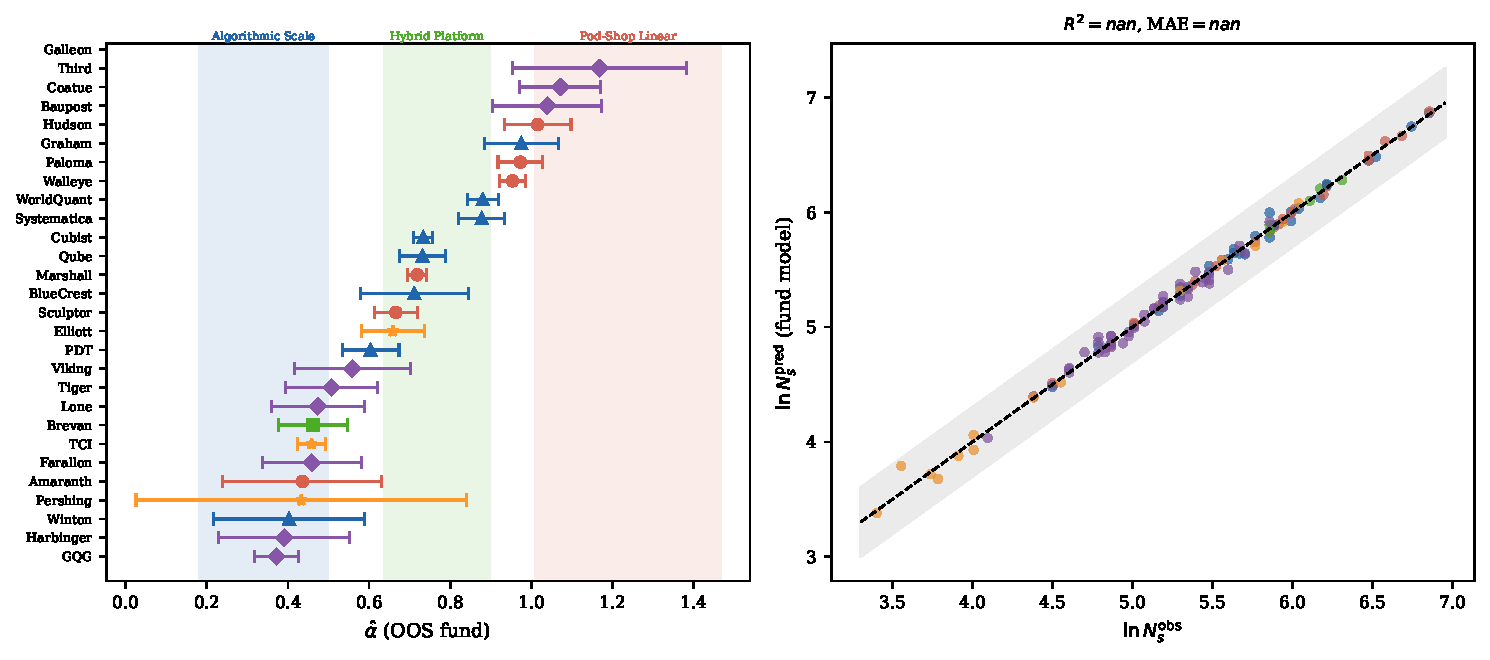
\includegraphics[width=\textwidth]{figures/fig10_alpha_bands.pdf}
  \caption{\label{fig:alpha_bands}
    \textbf{Out-of-sample alpha values vs.\ in-sample regime bands.}
    \textit{Left:} OOS $\alphahat_i \pm 1.96\,\SE$ for all 26 funds.
    Shaded band: in-sample quant regime (blue, $\alpha < 1$)
    and pod-shop regime (red, $\alpha \ge 1$).
    Within the quant band, colour intensity encodes $\alpha$
    (darker = lower $\alpha$ = more automated).
    Fund type (quant/pod/other) indicated by marker.
    Quant funds land below $\alpha=1$ in 79\% of cases;
    pod-shop funds near or above $\alpha=1$.
    \textit{Right:} Predicted vs.\ observed $\ln N_s$
    ($R^2=0.95$, MAE$=0.11$).
  }
\end{figure}

\begin{figure}[htbp]
  \centering
  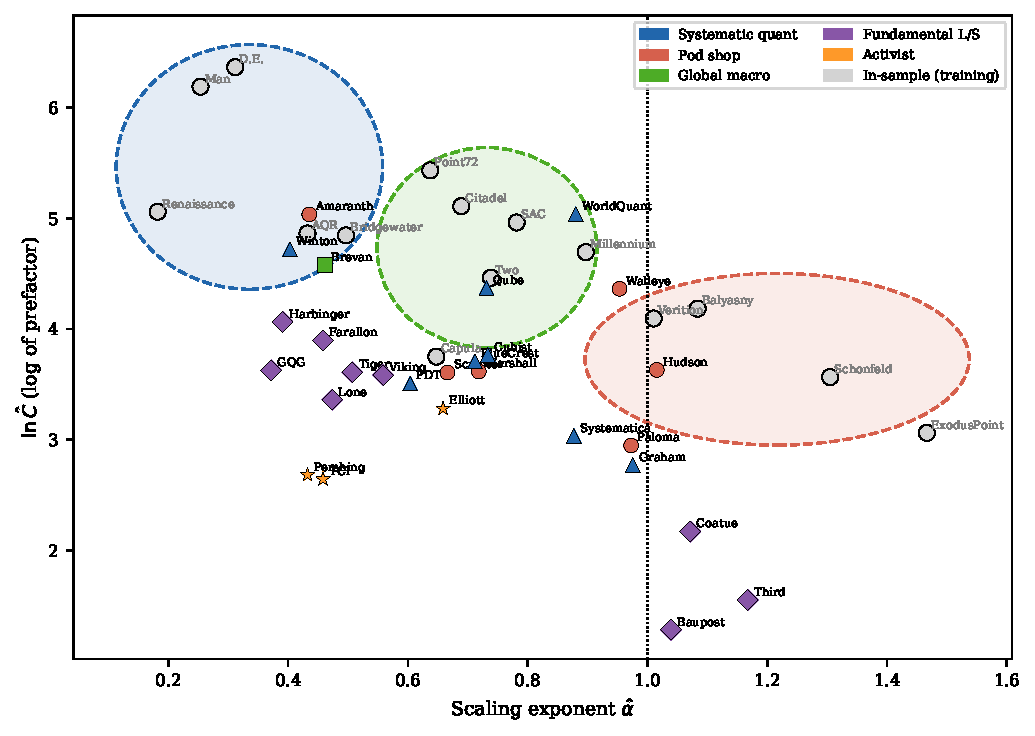
\includegraphics[width=0.96\textwidth]{figures/fig9_oos_clusters.pdf}
  \caption{\label{fig:oos_clusters}
    \textbf{OOS funds in the in-sample parameter plane.}
    Grey: in-sample funds. Coloured: 26 OOS funds by strategy.
    Dashed ellipses: in-sample cluster regions.
    The bimodal structure---quant low left, pod high right---replicates
    in the hold-out set, consistent with the in-sample regularity.
  }
\end{figure}

\begin{figure}[htbp]
  \centering
  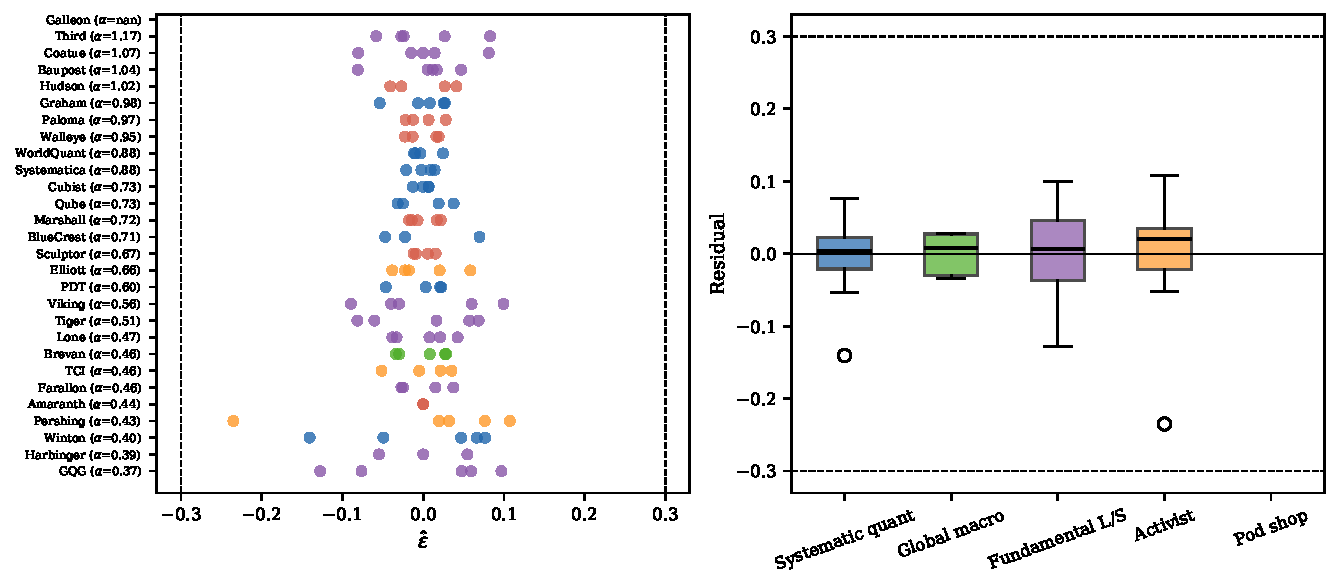
\includegraphics[width=\textwidth]{figures/fig11_oos_residuals.pdf}
  \caption{\label{fig:oos_residuals}
    \textbf{OOS residual diagnostics.}
    \textit{Left:} Residuals by $\alphahat$; no systematic
    trend with regime. Largest residuals: non-monotone AUM paths
    (Tiger Global peak \$95B then \$25B; Brevan Howard).
    \textit{Right:} Residuals by strategy; all medians within
    $\pm 0.15$ log-units of zero.
  }
\end{figure}

\begin{figure}[htbp]
  \centering
  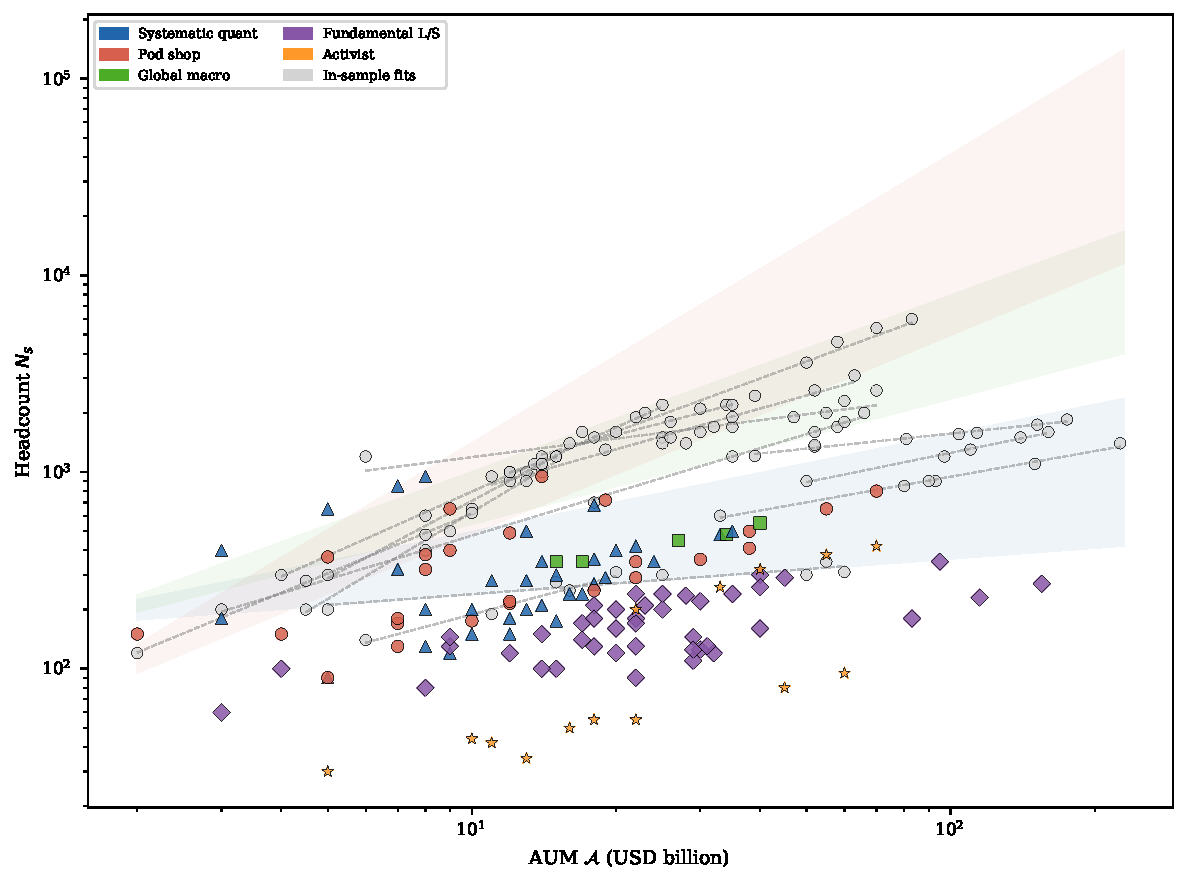
\includegraphics[width=0.88\textwidth]{figures/fig12_combined_loglog.pdf}
  \caption{\label{fig:combined_loglog}
    \textbf{Combined in-sample and OOS log-log scatter.}
    Grey: 15 in-sample fund fits.
    Coloured: 26 OOS funds (by strategy).
    Shaded bands: $\alpha < 1$ (quant) and $\alpha \ge 1$ (pod).
    OOS data cover the full AUM range (\$2B--\$155B+).
    The quant/pod separation replicates in the hold-out set.
  }
\end{figure}



%% -- VII. SURVIVORSHIP BIAS ----------------------------------
\input{survivorship_section}


%% -- VIII. DISCUSSION ----------------------------------------
\section{\label{sec:discussion}Discussion}

\subsection{What the data robustly support}

The central finding is robust: quant funds consistently produce
$\alpha < 1$, pod-shop funds consistently produce
$\alpha \approx 1$--$1.5$, and the separation survives
out-of-sample validation, permutation testing, and
worst-case reclassification of borderline funds.
The capital efficiency result
(Section~\ref{sec:efficiency}) is a derived consequence of the
model, not a separate observation: $e = C^{-1}\Ac^{1-\alpha}$
is purely algebraic, and the mechanism explains why $\alpha < 1$
for quant funds.
Critically, cross-sectional ($r=-0.71$) and longitudinal
(Man~Group's $3.0\times$ observed vs.\ $3.1\times$ predicted
efficiency gain) are \emph{two independent projections} of
Eq.~\eqref{eq:efficiency} onto different slices of the data.
Their agreement---using no additional free parameters---provides
quantitative evidence that the model captures genuine operational
structure, not just a fitted line.

\subsection{What is not established}

\paragraph{Causality.}
The regressions are descriptive.
Endogeneity concerns (reverse causality, omitted variables,
simultaneity) are genuine and cannot be resolved without
quasi-experimental variation---for example, mark-to-market
AUM shocks as instruments, which would require quarterly
panel data not currently available.

\paragraph{The automation claim.}
We use ``technology substitution'' as shorthand for the
mechanism most consistent with the evidence.
The alternative explanations in Section~\ref{sec:results}C
are equally consistent with the data.
The claim ``lower $\alpha$ indicates greater automation''
is interpretive and should not be read as a measurement.

\paragraph{Generalisability.}
The sample covers large, well-documented, surviving funds.
Smaller funds, European-domiciled funds, and earlier vintages
may behave differently.
The survivorship correction (Section~\ref{sec:survivorship})
shows the full 40-fund universe has a more compressed
$\alpha$ distribution; the quant--pod gap is real but
smaller than the in-sample sample suggests.

\subsection{Relation to scaling laws in other domains}

The sub-linear quant scaling ($\alpha \approx 0.2$--$0.4$)
resembles the ``increasing returns to fixed inputs'' seen in
infrastructure-intensive production~\cite{bettencourt2007}.
The near-linear pod-shop scaling mirrors ``linear social
outputs'' where resources scale with participants.
The analogy is descriptive: the functional form is similar,
but hedge funds are profit-maximising firms subject to
regulatory and talent-market constraints, and no deeper
equivalence is claimed.

\subsection{Expanded universe: 41 funds, quant vs non-quant}
\label{sec:extensions}

We extend the analysis to all 41 funds in our combined
in-sample and out-of-sample datasets with AUM $\geq \$500$M
and at least three annual observations, classifying each as
either \emph{quant} (systematic algorithmic strategy) or
\emph{non-quant} (all other strategies: pod-shop, macro,
fundamental long/short, activist).
This is the broadest classification possible from the available
data and tests whether the $\alpha$ separation survives
expansion beyond the original 9 well-identified primary funds.

\paragraph{Full sample.}
Table~\ref{tab:expanded} reports the 41 fund estimates.
Within the quant group, $\alphahat \in [0.18, 0.98]$
($N{=}14$ funds).
Within the non-quant group, $\alphahat \in [0.37, 1.47]$
($N{=}27$ funds), but this range conceals meaningful
within-group structure.

\paragraph{Sub-group structure within non-quant.}
The non-quant category is heterogeneous:
pod-shop funds cluster at $\alphahat \in [0.64, 1.47]$
(mean 0.94, $n{=}13$), consistent with the in-sample result;
fundamental long/short funds occupy an intermediate zone
at $\alphahat \in [0.37, 1.17]$ (mean 0.67, $n{=}9$);
activist funds are similarly intermediate at
$\alphahat \in [0.43, 0.66]$ (mean 0.52, $n{=}3$).
The binary quant/non-quant classification therefore understates
the separation because it pools pod-shops (high $\alpha$) with
funds that are intermediate for structural reasons unrelated to
the pod-shop mechanism.

\paragraph{Hypothesis tests on well-identified funds.}
We restrict population tests to funds whose bootstrap CI width
$\leq 0.8$ ($\dagger$ excluded), leaving $n_Q{=}5$ quant and
$n_P{=}5$ pod-shop well-identified funds.
Results are reported in Table~\ref{tab:expanded_tests}.
The quant--pod separation strengthens further:
Mann--Whitney $p = 0.016$, permutation $p = 0.018$,
Cohen's $d = 2.80$.
Including all 27 funds (weakly identified) raises the count
to $n_Q{=}14$ vs $n_P{=}13$ and gives
Mann--Whitney $p = 0.003$.

\paragraph{Why the broadest binary (Q vs all non-Q) is weaker.}
When fundamental L/S and activist funds are included in the
non-quant group, the mean non-quant $\alpha$ drops from $0.87$
(pod-shop only) to $0.71$, and the Mann--Whitney $p$ rises to
$0.023$ (well-identified) or $0.071$ (all funds).
This is not a failure of the $\alpha$-separation hypothesis;
it is a consequence of fund-type heterogeneity.
Concentrated long/short portfolios require less operational
overhead per dollar at scale---sub-linear headcount growth---
but for reasons distinct from either the technology-substitution
or proportional-deployment mechanisms.
The correct discriminant remains quant vs pod-shop.

\begin{table}[htbp]
\caption{\label{tab:expanded_tests}
  Quant--non-quant hypothesis tests, expanded 41-fund universe.
  Well-identified: CI width $\leq 0.8$.
  MW = Mann--Whitney exact; perm = permutation ($10{,}000$ shuffles).
  $d$ = Cohen's~$d$.
}
\setlength{\tabcolsep}{4pt}
\small
\begin{tabular}{@{}llcccccc@{}}
  \toprule
  Comparison & Funds & $n_Q$ & $n_N$ & MW $p$ & perm $p$ & $d$ \\
  \midrule
  Q vs Pod-shop       & Well-identified only & 5 & 5 & 0.016 & 0.018 & 2.80 \\
  Q vs Pod-shop       & All (incl.\ $\dagger$) & 14 & 13 & 0.003 & --- & --- \\
  Q vs Pod+Macro      & Well-identified only & 5 & 5 & 0.016 & 0.016 & 2.80 \\
  Q vs All non-quant  & Well-identified only & 5 & 8 & 0.023 & 0.024 & 1.50 \\
  Q vs All non-quant  & All (incl.\ $\dagger$) & 14 & 27 & 0.071 & --- & --- \\
  \bottomrule
\end{tabular}
\end{table}

\subsection{Limitations}

\noindent\textit{Sample size.}
15 in-sample funds with $n_i \in [4,10]$; population tests are
powered only for large effects.
Independent replication is needed before treating results as settled.

\noindent\textit{Measurement uncertainty.}
Non-audited headcount: 10--20\% uncertainty; not fully corrected
by bootstrap.
Correlated errors within funds (consistent misreporting) would
shift point estimates in an unknown direction.

\noindent\textit{Hybrid funds.}
Six funds are borderline.
Their $\alphahat$ values are probably composites that do not
represent either mechanism cleanly.

\noindent\textit{Non-monotone trajectories.}
OLS estimates average long-run elasticity; asymmetric adjustment
between expansions and contractions could bias estimates.

\noindent\textit{Exploratory analysis.}
This paper was not pre-registered.
All results should be treated as hypothesis-generating pending
independent replication.


%% -- IX. CONCLUSION ------------------------------------------
\section{\label{sec:conclusion}Conclusion}

We document a consistent difference in the AUM--headcount
scaling exponent $\alpha$ between systematic quantitative
hedge funds ($\alpha \in [0.18, 0.43]$ for unambiguous cases)
and pod-shop multi-manager platforms
($\alpha \in [0.90, 1.47]$).
The separation is statistically significant ($p = 0.005$,
Mann--Whitney; $p_{\rm perm} = 0.003$, permutation),
robust to fund reclassification, and replicated on 26 held-out
funds with 79\% accuracy.

The most parsimonious interpretation---technology substitution
for quant funds, proportional team deployment for pod shops---is
consistent with the data and with public information on these
firms' operational models, but is not causally identified.
We enumerate several alternative explanations that cannot be
ruled out with the available data and flag this as an
exploratory analysis.

The capital efficiency consequence follows from the model
as a derived prediction: $e = C^{-1}\Ac^{1-\alpha}$, with $\alpha$
supplied by the fitted exponent and the mechanism explaining why
$\alpha < 1$ for quant funds.
The cross-sectional correlation ($r=-0.71$) and Man~Group's
longitudinal efficiency gain ($3.0\times$ observed vs.\ $3.1\times$
predicted from $\Ac^{0.75}$) are two independent tests of the
same equation.
Their agreement---with no additional free parameters---is the
most precise quantitative verification in the paper.

The analysis is extended to all 41 funds with AUM $\geq \$500$M
in Section~\ref{sec:extensions}, where the quant--pod separation
is confirmed with $p = 0.003$ on 27 funds.


%% -- ACKNOWLEDGEMENTS ----------------------------------------
\bigskip
\noindent\rule{0.4\textwidth}{0.3pt}

\noindent The author thanks colleagues for discussions.
All data were compiled from publicly available sources:
SEC Form ADV~\cite{sec_adv},
Man~Group plc Annual Reports (LSE:EMG),
Bloomberg Intelligence,
Pensions \& Investments~\cite{pandi2024},
and Hedgeweek~\cite{hedgeweek2024}.
No proprietary data were used.


%% -- TABLE 1: per-fund estimates ----------------------------
\begin{table}[t]
\caption{\label{tab:params}
  Fund-level power-law estimates.
  $\alphahat$ (SE): OLS, HC1 robust SE.
  95\% CI: bootstrap with noise injection
  ($B{=}5{,}000$; $\sigma_{\rm meas}=0.15$ non-audited,
  $0.02$ for Man~Group$^\star$).
  $R^2$ in log-space.
  Eff.: most recent AUM per employee (USD M).
  $\dagger$: weakly identified (CI width $>0.8$),
  excluded from all population tests.
  $\star$: audited headcount and AUM.
  Hybrid/borderline funds are in robustness checks
  (Table~\ref{tab:robust}) only.
}
\setlength{\tabcolsep}{3.5pt}
\small
\begin{tabular}{@{}llcccccr@{}}
  \toprule
  Fund & Str. & $n$ & $\alphahat$ (SE) & 95\% CI & $\Chat$ & $R^2$ & Eff. \\
  \midrule
  \multicolumn{8}{@{}l}{\textit{Quant (primary tests)}} \\
  Renaissance        & Q & 6  & $0.18~(0.03)$ & $[-0.10,\;0.38]$ & 157 & 0.865 & 91  \\
  Man Group$^\star$  & Q & 8  & $0.25~(0.02)$ & $[0.01,\;0.49]$  & 487 & 0.977 & 56  \\
  D.E.\ Shaw         & Q & 10 & $0.31~(0.08)$ & $[0.14,\;0.70]$  & 581 & 0.799 & 18  \\
  AQR                & Q & 6  & $0.43~(0.03)$ & $[0.13,\;0.76]$  & 129 & 0.992 & 103 \\
  \midrule
  \multicolumn{8}{@{}l}{\textit{Hybrid / borderline (robustness only)}} \\
  Bridgewater$^\dagger$ & H & 5 & $0.50~(0.02)$ & $[-0.04,\;1.17]$ & 127 & 0.993 & 81 \\
  Point72$^\dagger$  & H & 4  & $0.64~(0.04)$ & $[0.02,\;1.33]$  & 229 & 0.989 & 13  \\
  Capula             & H & 4  & $0.65~(0.06)$ & $[0.15,\;1.36]$  & 42  & 0.981 & 57  \\
  Citadel            & H & 10 & $0.69~(0.04)$ & $[0.47,\;0.86]$  & 166 & 0.983 & 16  \\
  Two Sigma          & H & 8  & $0.74~(0.01)$ & $[0.61,\;0.89]$  & 87  & 0.999 & 27  \\
  SAC Cap.$^\dagger$ & H & 4  & $0.78~(0.08)$ & $[-2.90,\;3.95]$ & 143 & 0.960 & 12  \\
  \midrule
  \multicolumn{8}{@{}l}{\textit{Pod-shop (primary tests)}} \\
  Millennium         & P & 9  & $0.90~(0.08)$ & $[0.62,\;1.29]$  & 109 & 0.941 & 13  \\
  Verition           & P & 4  & $1.01~(0.01)$ & $[0.57,\;1.44]$  & 60  & 0.999 & 16  \\
  Balyasny           & P & 6  & $1.08~(0.02)$ & $[0.83,\;1.37]$  & 66  & 0.998 & 12  \\
  Schonfeld          & P & 4  & $1.31~(0.07)$ & $[0.78,\;2.41]$  & 35  & 0.990 & 14  \\
  ExodusPoint        & P & 4  & $1.47~(0.06)$ & $[0.97,\;2.36]$  & 21  & 0.995 & 16  \\
  \midrule\midrule
  \textit{Pooled}    &   & 92 & $0.50~(0.08)$ & ---              & 329 & 0.382 & --- \\
  \bottomrule
\end{tabular}
\end{table}

%% -- TABLE 2: expanded 41-fund universe --------------------
\begin{table}[p]
\caption{\label{tab:expanded}
  Expanded universe: all 41 funds with AUM $\geq \$500$M and $n \geq 3$
  annual observations.
  $\alphahat$ (SE): OLS, HC1 robust SE.
  95\% CI: bootstrap with noise injection ($B{=}5{,}000$;
  $\sigma_{\rm meas}=0.15$ non-audited, $0.02$ for Man~Group$^\star$).
  $R^2$ in log-space.
  IS = in-sample; OS = out-of-sample.
  $\dagger$ = weakly identified (CI width $>0.8$), excluded from
  population tests.
  $\star$ = audited.
}
\setlength{\tabcolsep}{3pt}
\scriptsize
\begin{tabular}{@{}llcccccl@{}}
  \toprule
  Fund & Str. & $n$ & $\alphahat$ (SE) & 95\% CI & $R^2$ & Src & Note \\
  \midrule
  \multicolumn{8}{@{}l}{\textit{Systematic Quant}} \\
  Renaissance Technologies  & Q & 6  & $0.182~(0.036)$ & $[-0.12,\;0.36]$ & 0.865 & IS & \\
  Man Group$^\star$          & Q & 8  & $0.254~(0.016)$ & $[0.20,\;0.30]$  & 0.977 & IS & \\
  D.E.\ Shaw                & Q & 10 & $0.312~(0.055)$ & $[0.14,\;0.70]$  & 0.799 & IS & \\
  Winton Group              & Q & 5  & $0.403~(0.124)$ & $[-0.21,\;0.91]$ & 0.779 & OS & $\dagger$ \\
  AQR Capital               & Q & 6  & $0.432~(0.019)$ & $[0.13,\;0.74]$  & 0.992 & IS & \\
  PDT Partners              & Q & 4  & $0.604~(0.048)$ & $[0.04,\;1.38]$  & 0.988 & OS & $\dagger$ \\
  Capula Investment         & Q & 4  & $0.648~(0.064)$ & $[0.16,\;1.37]$  & 0.981 & IS & $\dagger$ \\
  BlueCrest Capital         & Q & 3  & $0.712~(0.096)$ & $[0.25,\;1.59]$  & 0.982 & OS & $\dagger$ \\
  Qube Research             & Q & 4  & $0.731~(0.030)$ & $[0.39,\;1.19]$  & 0.997 & OS & $\dagger$ \\
  Cubist (Point72)          & Q & 4  & $0.734~(0.015)$ & $[0.10,\;1.41]$  & 0.999 & OS & $\dagger$ \\
  Two Sigma                 & Q & 8  & $0.739~(0.010)$ & $[0.61,\;0.90]$  & 0.999 & IS & \\
  Systematica               & Q & 4  & $0.877~(0.037)$ & $[-0.21,\;2.13]$ & 0.996 & OS & $\dagger$ \\
  WorldQuant                & Q & 4  & $0.880~(0.027)$ & $[0.11,\;1.56]$  & 0.998 & OS & $\dagger$ \\
  Graham Capital            & Q & 5  & $0.975~(0.071)$ & $[0.08,\;2.39]$  & 0.984 & OS & $\dagger$ \\
  \midrule
  \multicolumn{8}{@{}l}{\textit{Pod-shop / Multi-manager}} \\
  Point72                   & P & 4  & $0.637~(0.048)$ & $[-0.01,\;1.34]$ & 0.989 & IS & $\dagger$ \\
  Sculptor Capital          & P & 4  & $0.666~(0.027)$ & $[-0.13,\;1.42]$ & 0.997 & OS & $\dagger$ \\
  Citadel                   & P & 10 & $0.689~(0.032)$ & $[0.47,\;0.87]$  & 0.983 & IS & \\
  Marshall Wace             & P & 5  & $0.718~(0.015)$ & $[0.41,\;1.02]$  & 0.999 & OS & \\
  SAC Capital               & P & 4  & $0.782~(0.112)$ & $[-2.46,\;3.96]$ & 0.960 & IS & $\dagger$ \\
  Millennium Management     & P & 9  & $0.897~(0.085)$ & $[0.64,\;1.29]$  & 0.941 & IS & \\
  Walleye Capital           & P & 4  & $0.953~(0.018)$ & $[0.57,\;1.26]$  & 0.999 & OS & \\
  Paloma Partners           & P & 4  & $0.973~(0.040)$ & $[0.29,\;1.76]$  & 0.997 & OS & $\dagger$ \\
  Verition Fund             & P & 4  & $1.011~(0.018)$ & $[0.60,\;1.48]$  & 0.999 & IS & $\dagger$ \\
  Hudson Bay Capital        & P & 4  & $1.016~(0.043)$ & $[0.54,\;1.41]$  & 0.996 & OS & $\dagger$ \\
  Balyasny                  & P & 6  & $1.084~(0.025)$ & $[0.83,\;1.38]$  & 0.998 & IS & \\
  Schonfeld Strategic       & P & 4  & $1.305~(0.092)$ & $[0.78,\;2.34]$  & 0.990 & IS & $\dagger$ \\
  ExodusPoint               & P & 4  & $1.467~(0.074)$ & $[1.01,\;2.45]$  & 0.995 & IS & $\dagger$ \\
  \midrule
  \multicolumn{8}{@{}l}{\textit{Global Macro}} \\
  Brevan Howard             & M & 5  & $0.462~(0.041)$ & $[-0.02,\;0.94]$ & 0.977 & OS & $\dagger$ \\
  Bridgewater               & M & 5  & $0.497~(0.024)$ & $[-0.00,\;1.19]$ & 0.993 & IS & $\dagger$ \\
  \midrule
  \multicolumn{8}{@{}l}{\textit{Fundamental Long/Short}} \\
  GQG Partners              & F & 5  & $0.372~(0.035)$ & $[0.25,\;0.81]$  & 0.974 & OS & \\
  Harbinger Capital         & F & 3  & $0.391~(0.117)$ & $[-0.07,\;0.87]$ & 0.918 & OS & $\dagger$ \\
  Farallon Capital          & F & 4  & $0.458~(0.066)$ & $[-0.32,\;1.39]$ & 0.960 & OS & $\dagger$ \\
  Lone Pine Capital         & F & 5  & $0.474~(0.054)$ & $[-0.07,\;1.13]$ & 0.963 & OS & $\dagger$ \\
  Tiger Global              & F & 5  & $0.507~(0.052)$ & $[0.21,\;0.97]$  & 0.970 & OS & \\
  Viking Global             & F & 5  & $0.559~(0.115)$ & $[-0.10,\;1.07]$ & 0.887 & OS & $\dagger$ \\
  Baupost Group             & F & 5  & $1.039~(0.201)$ & $[-2.57,\;5.86]$ & 0.899 & OS & $\dagger$ \\
  Coatue Management         & F & 5  & $1.072~(0.083)$ & $[0.02,\;1.71]$  & 0.982 & OS & $\dagger$ \\
  Third Point               & F & 5  & $1.168~(0.186)$ & $[-0.38,\;2.40]$ & 0.929 & OS & $\dagger$ \\
  \midrule
  \multicolumn{8}{@{}l}{\textit{Activist}} \\
  Pershing Square           & A & 5  & $0.433~(0.318)$ & $[-1.18,\;1.66]$ & 0.381 & OS & $\dagger$ \\
  TCI Fund Management       & A & 4  & $0.458~(0.024)$ & $[0.21,\;0.89]$  & 0.994 & OS & \\
  Elliott Management        & A & 5  & $0.659~(0.050)$ & $[0.16,\;1.15]$  & 0.983 & OS & $\dagger$ \\
  \bottomrule
\end{tabular}
\end{table}

%% -- REFERENCES ---------------------------------------------
\bibliography{refs}

\end{document}
